% Tema4.tex

\chapter{Variedades topológicas. Superficies}

\section{La topología cociente}

\defn{Topología final o imagen}{
    Sea \((X, \T)\) un espacio topológico, \(Y\) un conjunto y \(p: X \to Y\) una aplicación. Definimos en \(Y\) la topología final o imagen de \(p\) como:
    \[
    \T(p) := \{O \subset Y \mid p^{-1}(O) \in \T\}.
    \]
}
\clmp{}{
    $\T(p)$ es una topología sobre $Y$
}{
    \begin{enumerate}
    \item[(T1)] $p^{-1}(\emptyset)=\emptyset\in\T\implies\emptyset\in\T(p)$. $p^{-1}(Y)=X\in\T\implies Y\in\T(p)$.
    \item[(T2)] Si $U_i\in\T(p)\ \forall i\in I$ entonces $p^{-1}(U_i)\in\T\ \forall i\in I$, por tanto $p^{-1}(\bigcup_{i\in I}U_i)=\bigcup_{i\in I}p^{-1}(U_i)\in\T$ lo que significa que $\bigcup_{i\in I}U_i\in\T(p)$.
    \item[(T3)] Si $U_i\in\T(p)\ \forall i\in\{1,\dots,n\}$ entonces $p^{-1}(U_i)\in\T\ \forall i\in\{1,\dots,n\}$, por tanto $p^{-1}(\bigcap_{i=1}^{n}U_i)=\bigcap_{i=1}^{n}p^{-1}(U_i)\in\T$ lo que significa que $\bigcap_{i=1}^{n}U_i\in\T(p)$.
    \end{enumerate}
}


\propp{Propiedades de la topología final}{\label{prop:112}
    \begin{enumerate}
    \item \(\T(p)\) hace a \(p\) continua y es la topología más fina que lo hace.
    \item Sea \(g : (Y, \T(p)) \to (Z, \T'')\) una aplicación. \(g\) es continua si y solo si \(g \circ p\) es continua.  
    \item Los cerrados de \(\T(p)\) son \(\{C \subset Y \mid p^{-1}(C) \text{ es cerrado en } \T\}\).
    \end{enumerate}
}{
    \begin{enumerate}
        \item Que $\T(p)$ hace continua a $p$ es inmediato por la propia definición de $\T(p)$. Además, si $\T'$ es otra topología cualquiera que hace a $p$ continua entonces $\forall U\in\T', p^{-1}(U)\in\T\implies U\in\T(p)$, por lo que $\T'\subset\T(p)$, luego la topología final es la más fina.
        \item Claramente si $g$ es continua entonces $g\circ p$ es continua, puesto que es composición de dos aplicaciones continuas (recordemos que $p$ es continua como aplicación en $(Y,\T(p))$). Si por el contrario $g\circ p$ es continua, entonces dado $U\in\T''$ arbitrario, la preimagen $(g\circ p)^{-1}(U)=p^{-1}(g^{-1}(U))\in\T$ es abierta por ser $g\circ p$ continua, pero entonces por la definición de $\T(p)$ debe cumplirse $g^{-1}(U)\in\T(p)$, por tanto $g$ es continua.
        \item $C$ es cerrado en $\T(p) \iff Y\setminus C\in\T(p)\iff p^{-1}(Y\setminus C)\in\T \iff X\setminus p^{-1}(C)\in\T\iff p^{-1}(C)$ es cerrado en $\T$. El tercer $\iff$ se cumple puesto que $p^{-1}(Y)=X$.
    \end{enumerate}
}

\defn{Identificación}{
    Sean \((X, \T)\), \((Y, \T')\) espacios topológicos, y \(p: X \to Y\) una aplicación. Decimos que \(p : (X, \T) \to (Y, \T')\) es una identificación si \(p\) es sobreyectiva y \(\T' = \T(p)\).
}

\rmkb{Si $f:X\to Y$ es una aplicación sobreyectiva entonces $f(f^{-1}(U))=U$ para cualquier $U\subset X$.}

\propp{Propiedades de las identificaciones}{\label{prop:114}
    \begin{enumerate}
    \item \(Id : (X, \T) \to (X, \T')\) es una identificación si y solo si \(\T = \T'\).  
    \item Si \(p : (X, \T) \to (Y, \T')\) es una identificación y \(f : (Y, \T') \to (Z, \T'')\) es una aplicación, entonces \(f\) es continua si y solo si \(f \circ p\) es continua.
    \item Si \(f : (X, \T) \to (Y, \T')\) es continua, abierta (o cerrada) y sobreyectiva, entonces \(f\) es una identificación.
    \end{enumerate}
}{
    \begin{enumerate}
        \item Claramente $Id$ es sobreyectiva (de hecho es biyectiva con inversa $(Id)^{-1}=Id$), por lo que será identificación si y solo si $\T'=\T(Id)$. Ahora bien, $\T(Id)=\{O \subset Y \mid (Id)^{-1}(O) \in \T\}=\{O \subset Y \mid O \in \T\}=\T$, por tanto $Id$ es identificación si y solo si $\T'=\T$.
        \item Si $f$ es continua entonces $f\circ p$ es continua por ser composición de aplicaciones continuas. Si por el contrario $f\circ p$ es continua, entonces dado $U\in\T''$ arbitrario, la preimagen $(f\circ p)^{-1}(U)=p^{-1}(f^{-1}(U))\in\T$ es abierta por ser $f\circ p$ continua, pero entonces, como $\T'=\T(p)$ al ser $p$ identificación, debe cumplirse $f^{-1}(U)\in\T'$, por tanto $f$ es continua.
        \item Como $f$ es sobreyectiva solo necesitamos ver que si es continua y abierta (cerrada) entonces $\T'=\T(f)$. Supongamos que $f$ es continua, en tal caso tenemos garantizado que $\T'\subset\T(f)$.
        
        Si además es abierta entonces dado $U\in\T(f)$ arbitrario, $f^{-1}(U)\in\T$ por la definición de $\T(f)$, pero entonces $f(f^{-1}(U))\in\T'$ al ser $f$ abierta, y como es sobreyectiva $f(f^{-1}(U))=U\in\T'$, por lo que $\T(f)\subset\T'\subset\T(f)\implies \T(f)=\T'$, luego $f$ es una identificación.
        
        Si $f$ es cerrada razonamos de manera similar pero con cerrados: dado $U\in\T(f)$, $C=Y\setminus U$ es cerrado en $\T(f)$, por lo que $f^{-1}(C)$ es cerrado en $\T$\footnote{Por la tercera parte de la Proposición \hyperref[prop:112]{1.1.2}}, por tanto $f(f^{-1}(C))=C$ es cerrado en $\T$ al ser $f$ cerrada, pero entonces $U=Y\setminus(Y\setminus C)\in\T$, por tanto $\T(f)\subset\T'\subset\T(f)\implies \T(f)=\T'$, luego $f$ es una identificación.
    \end{enumerate}
}

\defn{Topología cociente}{
    Sea \((X, \T)\) un espacio topológico, \(\sim\) una relación de equivalencia en \(X\), y \(p: X \to \faktor{X}{\sim} = \tilde{X}\) la proyección al cociente. La topología cociente sobre \(\tilde{X}\) es la topología final o imagen de $p$:
    \[
    \faktor{\T}{\sim} = \tilde{\T} := \T(p) = \{ V \subset \tilde{X} \mid p^{-1}(V) \in \T \}.
    \]
    El espacio \((\tilde{X}, \tilde{\T})=(\faktor{X}{\sim},\faktor{\T}{\sim})\) se llama espacio cociente.
}

% \clmp{}{
%     $\tilde{\T}$ es una topología sobre $\tilde{X}$
% }{
%     Trivial.
% }

\rmkb{
    \begin{enumerate}
        \item  Toda relación de equivalencia \(\sim\) sobre \(X\) determina un espacio cociente dado por \(\tilde{X} = X / \sim\). Recíprocamente, todo espacio final asociado a una aplicación $p$ es el espacio cociente correspondiente a la relación de equivalencia $\sim_p$ dada por
        
        $x\sim_py\iff p(x)=p(y)$.
        \item Al definir un cociente estamos identificando los puntos que están en una misma clase de equivalencia.
        \item  \(\tilde{\T}\) es la topología más fina sobre \(\tilde{X}\) que hace continua a \(p\).
    \end{enumerate}
}

\propp{Propiedades del espacio cociente}{\label{prop:116}
    \begin{enumerate}
    \item \(V\) es un abierto de \(\tilde{X}\) si y solo si \(\bigcup_{[x] \in V}[x]\) es abierto en \(X\).  
    \item Si \(X\) es compacto, entonces \(\tilde{X}\) es compacto.  
    \item Si \(X\) es conexo (conexo por caminos), entonces \(\tilde{X}\) es conexo (conexo por caminos).
    \item $p:(X,\T)\to(\tilde{X},\tilde{\T})$ es una identificación.
    \item \(g : (\tilde{X}, \tilde{\T}) \to (Y, \T')\) es continua si y solo si \(g \circ p : (X, \T) \to (Y, \T')\) es continua.
    \end{enumerate}
}{
    \begin{enumerate}
        \item $V\in\tilde{\T}\iff p^{-1}(V)\in\T$ por definición de la topología cociente, veamos que $p^{-1}(V)=\bigcup_{[x] \in V}[x]$. Si $y \in p^{-1}(V) \implies p(y)=[y] \in V$, por tanto $[y]\subset\bigcup_{[x] \in V}[x]$, luego $y\in[y]\subset\bigcup_{[x] \in V}[x]$, por lo que $p^{-1}(V)\subset\bigcup_{[x] \in V}[x]$.
        
        Por otro lado si $x\in\bigcup_{[x] \in V}[x]$ entonces $[x]\in V$, por tanto $p(x)=[x] \in V \implies x \in p^{-1}(V)$, lo que prueba finalmente que $p^{-1}(V)=\bigcup_{[x] \in V}[x]$.
        \item Supongamos que $X$ es compacto y sea $\mathcal{A}=\{A_i\}_{i \in I}$, por el apartado 1 los conjuntos $B_i=\bigcup_{[x] \in A_i}[x]$ son abiertos, y además recubren $X$ puesto que $\forall x \in X$, $[x] \in \tilde{X}$ por tanto $[x]\subset A_{i_0}$ para algún $i_0\in I$, luego $x\in B_{i_0}$. Por tanto $\{B_i\}_{i\in I}$ es un recubrimiento por abiertos de $X$, del que podemos extraer un subrecubrimiento finito $\{B_{i_1},\dots,B_{i_n}\}$ por la compacidad de $X$. Veamos ahora que $\{A_{i_1},\dots,A_{i_n}\}$ es un subrecubrimiento de $\tilde{X}$, para ello notemos que dado $[x]\in\tilde{X}, x\in B_{i_m}=\bigcup_{[x] \in A_{i_m}}[x]$ para cierto $m\in\{1,\dots,n\}$, por tanto $[x]\in A_{i_m}$, luego $\{A_{i_1},\dots,A_{i_n}\}$ es un subrecubrimiento finito y por tanto $\tilde{X}$ es compacto.
        \item Pendiente.
        \item Es inmediato que $\tilde{\T}=\T(p)$, por otro lado dado $y\in\tilde{\T}\implies y=[x]$ para cierto $x\in X$, por tanto $p(x)=y$, luego $p$ es sobreyectiva.
        \item Por el apartado 4, $p$ es una identificación, por tanto basta aplicar la parte 2 de la Proposición \hyperref[prop:114]{1.1.4}
    \end{enumerate}
}

Recordemos ahora que dada una aplicación $f:X\to Y$ cualquiera, podemos definir una relación de equivalencia sobre $X$ a partir de ella. Denotaremos por $R_f$ a la relación de equivalencia en $X$ dada por:
\[
x R_fx'\iff f(x)=f(x')
\]

\exer{
Demostrar que $R_f$ es una relación de equivalencia.
}


\thmr{Proposición 4.1}{diagrama}{
    Dados \((X, \T)\) y \((Y, \T')\) espacios topológicos y \((\tilde{X}, \tilde{\T})\) el espacio cociente dado por \(R_f\), existe una aplicación \(\tilde{f} : (\tilde{X}, \tilde{\T}) \to (Y, \T')\) que hace que el siguiente diagrama sea conmutativo\footnote{Que el diagrama sea conmutativo quiere decir que "da igual que camino de flechitas sigamos", es decir, $\tilde{f}\circ p=f$.}
    \begin{center}
        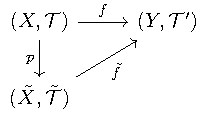
\includegraphics[]{otros/diagrama.pdf}
    \end{center}
    Además, \(f : (X, \T) \to (Y, \T)\) es una identificación si y solo si \(\tilde{f} : (\tilde{X}, \tilde{\T}) \to (Y, \T')\) es un homeomorfismo.
}
\pf{
    Si pretendemos que el diagrama sea conmutativo debe cumplirse
    \[
    \tilde{f}(p(x))=f(x)\iff \tilde{f}([x])=f(x)
    \]
    por tanto definimos $\tilde{f}$ de la siguiente manera:
    \[
    \tilde{f}:(\tilde{X}, \tilde{\T}) \to (Y, \T'),\quad \tilde{f}([x])=f(x).
    \]
    Ahora solo necesitamos ver que la aplicación está bien definida. En efecto si $x,y\in X$ son dos representantes de la misma clase de equivalencia $[x]$ entonces $xR_fy$, por tanto se cumple $f(x)=f(y)$, luego
    \[
    \tilde{f}([x])=f(x)=f(y)=\tilde{f}([y])
    \]
    por lo que la aplicación está bien definida\footnote{Está bien definida ya que hemos visto que la imagen de una clase de equivalencia no depende del representante escogido.}.

    Para la segunda parte, si suponemos que $\tilde{f}$ es un homeomorfismo entonces $f=\tilde{f}\circ p$ es continua por ser composición de funciones continuas, y es sobreyectiva por serlo $\tilde{f}$ y $p$. Además, si $U\in\T(f)$ entonces $f^{-1}(U)=p^{-1}(\tilde{f}^{-1}(U))\in\T$, por tanto $\tilde{f}^{-1}(U)\in\tilde{\T}$, y al ser $\tilde{f}$ abierta y biyectiva  $U=\tilde{f}(\tilde{f}^{-1}(U))\in\T'$, lo que prueba que $\T(f)=\T'$ y por tanto $f$ es una identificación.

    Si por el contrario suponemos que $f$ es una identificación entonces $f$ es sobreyectiva y $\T'=\T(f)$, por tanto $f$ es continua y al ser $p$ identificación también lo es $\tilde{f}$ (apartado 2 de la Proposición \hyperref[prop:114]{1.1.4}). Que $\tilde{f}$ es inyectiva es inmediato por  la propia definición de $\tilde{f}$. Para ver que es sobreyectiva, dado $y\in Y$ por ser $f$ sobreyectiva existe $x\in X\mid f(x)=y$, por tanto $\exists z=[x]\in\tilde{X}$ tal que $\tilde{f}([x])=f(x)=y$. Veamos que $\tilde{f}$ es abierta: dado $U\in\tilde{\T}$ entonces $f^{-1}(\tilde{f}(U))=p^{-1}(\tilde{f}^{-1}(\tilde{f}(U)))=p^{-1}(U)\in\T$ por ser $p$ continua, por lo tanto $\tilde{f}(U)\in\T(f)=\T'$, luego $\tilde{f}$ es un homeomorfismo.
}

\clearpage

\section{Ejemplos de espacios cocientes}

Veamos ahora algunos ejemplos de espacios cociente y su utilidad para encontrar homeomorfismos entre espacios topológicos. En estos primeros ejemplos haremos uso del Teorema \ref{thm:diagrama} para encontrar un homeomorfismo.
\\

\ex{
    Para el intervalo \(I = [0, 1]\), consideramos la partición:
    \[
    \tilde{I} = \{ \{0, 1\} \} \cup \{ \{x\} : x \in (0, 1) \}.
    \]
    El espacio cociente \((\tilde{I}, \tilde{\T})\) es homeomorfo a la circunferencia unidad \( \sphere^1 \).
}
\pf{
    Probemos que la relación $\sim$ dada por la partición $\tilde{I}$ coincide con la relación dada por la aplicación $f:I\to\sphere^1, f(t)=(\cos(2\pi t),\sin(2\pi t))$. Para ello, dados $x,y\in I$
    \[
    x R_f y \iff f(x)=f(y) \iff
    \begin{cases}
    \cos(2\pi x)=\cos(2\pi y)\\
    \sin(2\pi x)=\sin(2\pi y)
    \end{cases}
    \]
    Para que se den estas igualdades entre cosenos y senos hay varias opciones: si $x,y\in(0,1)$ entonces debe cumplirse $x=y$; si $x,y\in\{0,1\}$ entonces o bien $x=y$, o bien $x=0,y=1$, o bien $x=1,y=0$. En resumen:
    \[
    x R_f y \iff x=y \text{  o  } x=1,y=0 \text{  o  } x=0,y=1\iff x\sim y 
    \]
    Por tanto ambas son la misma relación. Ahora veamos que $f$ es una identificación, y por tanto $\exists \tilde{f}$ homeomorfismo entre $\tilde{I}$ y $\sphere^1$.

    En primer lugar, $f$ es continua por ser restricción de una aplicación continua (basta considerarla como aplicación de $I$ a $\R^2$), además es cerrada puesto que $I$ es compacto y $\sphere^2$ es Hausdorff (Ver Ejercicio \hyperref[exer:12]{1.2}). Por último dado $(x,y)\in\sphere^1$, si $(x,y)=(0,1)$ entonces $f(\frac{1}{4})=(0,1)=(x,y)$, si $(x,y)=(0,-1)$ entonces $f(\frac{3}{4})=(0,-1)=(x,y)$, si por el contrario $x\ne0$ entonces $\alpha=\frac{\arctan(\frac{y}{x})}{2\pi}$ verifica $f(\alpha)=(x,y)$. Por tanto $f$ es sobreyectiva, lo que según la Proposición \hyperref[prop:114]{1.1.4} apartado 3 garantiza que $f$ es una identificación, y por tanto $\exists \tilde{f}$ homeomorfismo entre $\tilde{I}$ y $\sphere^1$
}

\exer{Probar que si $X$ es compacto, $Y$ es Hausdorff y $f:(X,\T)\to(Y,\T')$ es continua entonces $f$ es cerrada.}\label{exer:12}


\ex{
    Sea \(X = [0, 1] \times [0, 1]\) con la relación de equivalencia:
    \[
    (x_1, y_1) \sim (x_2, y_2) \text{ si y solo si } x_1 - x_2 \in \mathbb{Z} \text{ e } y_1 = y_2.
    \]
    El espacio cociente es homeomorfo a un cilindro.
}

\ex{
    Sea \(X = [0, 1] \times [0, 1]\) con la relación de equivalencia:
    \[
    (x_1, y_1) \sim (x_2, y_2) \text{ si y solo si } (x_1, y_1) = (x_2, y_2) \text{ o } [x_1 - x_2 = \pm 1 \text{ e } y_1 = 1 - y_2].
    \]
    El espacio cociente es homeomorfo a una banda de Möbius.
}

\ex{
    Sea \(X = [0, 1] \times [0, 1]\) con la relación de equivalencia:
    \[
    (x_1, y_1) \sim (x_2, y_2) \text{ si y solo si } x_1 - x_2 \in \mathbb{Z} \text{ e } y_1 - y_2 \in \mathbb{Z}.
    \]
    El espacio cociente es homeomorfo a un toro.
}

\ex{
    Sea \(X = [0, 1] \times [0, 1]\) con la relación de equivalencia:
    \[
    (x_1, y_1) \sim (x_2, y_2) \text{ si y solo si } [x_1 = x_2 \text{ e } y_1 - y_2 \in \mathbb{Z}] \text{ o } [x_1 - x_2 = \pm 1 \text{ e } y_1 = 1 - y_2].
    \]
    El espacio cociente es homeomorfo a una botella de Klein.
}

\ex{
    Sea \(X = \mathbb{S}^1 \times [0, 1]\) con la relación de equivalencia:
    \[
    (x_1, y_1) \sim (x_2, y_2) \text{ si y solo si } y_1 = y_2 = 0 \text{ o } (x_1, y_1) = (x_2, y_2).
    \]
    El espacio cociente es homeomorfo a un cono.
}

\newpage

\ex{
    Sea \(X = \mathbb{S}^2\) con la relación de equivalencia:
    \[
    p \sim q \iff p = \pm q.
    \]
    El espacio cociente es homeomorfo al plano proyectivo \(\R\mathbb{P}^2\).
}

\ex{
    En el disco cerrado \(D(0, 1)\) de \(\mathbb{R}^2\), consideramos la relación de equivalencia:
    \[
    (x_1, y_1) \sim (x_2, y_2) \text{ si y solo si } x_1 = \pm x_2 \text{ e } y_1 = y_2.
    \]
    El espacio cociente \(\faktor{D(0, 1)}{\sim}\) es homeomorfo a la esfera \(\mathbb{S}^2\).
}

\exer{
Dado $(X,\T)$ un espacio topológico y $K\subset X$, definimos la relación
  \[
  x \sim y\iff
  \begin{cases}
    x,y \in K \\
    x=y
  \end{cases}
  \]
y llamemos al espacio cociente $(\faktor{X}{K},\faktor{\T}{K}):=(\faktor{X}{\sim},\faktor{\T}{\sim})$.
  \begin{enumerate}
    \item[a)] Demostrar que $p|_{X\setminus K}:X\to\faktor{X}{K}$ restringida a $p(X\setminus K)$ es una biyección.
    \item[b)] Demostrar que $p|_{X\setminus K}$ es un homeomorfismo si $K$ es abierto o cerrado.
  \end{enumerate}
}
\noindent\textbf{Solución:}

  Para simplificar la notación llamemos $f:=p|_{X\setminus K}$, y notemos que $\forall x \in X \setminus K, f(x)=[x]$, pero por la manera en la que está definida la relación de equivalencia, es inmediato ver que $[x]=\{x\}$, ya que el único elemento relacionado con $x$ es el propio $x$ (recordemos que $x\notin K$). Por tanto la inversa de $f$ es $f^{-1}([x])=x$, ya que $f(f^{-1}([x]))=f(x)=[x], f^{-1}(f(x))=f^{-1}([x])=x$ lo que prueba que $f$ es una biyección.
  
  ¿El apartado b) no es inmediato?
  % Para el apartado b) notemos en primer lugar que $p$ es continua, por lo que $f$ también lo será por ser su restricción. Si $K$ es abierto entonces $X\setminus K$ es cerrado, ahora si tomamos $U\in\T|_{X\setminus K}$ entonces $U=V\cap X\setminus K, V\in\T$, para ver que $f(U)$ es abierto, basta ver que $f^{-1}(f(U))
  % 
  % es cerrada, ya que dado $C$ cerrado en $X\setminus K$ se tiene
  % \[
  % f(C)=\bigcup_{[x]\in C}\{x\}
  % \]


\clearpage

\section{Espacios localmente euclídeos}

\defn{Espacio localmente euclídeo}{
    Un espacio topológico \((X, \T)\) se dice que es localmente euclídeo de dimensión \(n\) si todo punto \(p\) de \(X\) tiene un entorno \(U\) homeomorfo a una bola abierta \(B\) de \(\mathbb{R}^n\). Si \(\varphi: U \subset X \to B \subset \mathbb{R}^n\) es tal homeomorfismo, \((U, \varphi)\) se llama carta en \(X\) alrededor de \(p \in U\).
}

\rmkb{
    \begin{enumerate}
        \item Por ser \(X\) localmente euclídeo, este hereda las propiedades locales de \(\mathbb{R}^n\).
        \item Podemos sustituir la bola abierta en la definición anterior por un entorno abierto de \(\mathbb{R}^n\).
    \end{enumerate}
}

\defn{Bola euclídea}{
    Diremos que \(B' \subset X\) es una bola euclídea si $B'$ es homeomorfo a una bola abierta $B(0,r)$ de $\R^n$.
}

\defn{Bola regular euclídea}{
    Diremos que \(B \subset X\) es una bola regular euclídea si:
    \begin{itemize}
        \item Existe una bola euclídea \(B'\) tal que \(\overline{B} \subset B'\).
        \item Existe \(r > 0\) y una carta \(\varphi: B' \to B^n(0, 2r)\) tal que \(\varphi(\overline{B}) = B^n(0, r)\).
    \end{itemize}
}

\section{Variedades topológicas}

\defn{Variedad topológica}{
    Una variedad topológica \(M\) es un espacio topológico \(T_2\) y \(2A\N\) que es localmente euclídeo. La dimensión de \(M\) es el número natural \(n\). También se denomina \(n\)-variedad (topológica).
}

\defn{Superficie topológica}{
    Una superficie topológica \(S\) es una variedad topológica de dimensión dos o 2-variedad.
}

\defn{Variedad con borde}{
    Si en la definición de variedad cambiamos el espacio modelo \(\mathbb{R}^n\) por el semiespacio superior \(\mathbb{H}^n = \{x \in \mathbb{R}^n : x_i \geq 0\}\), obtenemos el concepto de variedad con borde.
}

\propp{Observaciones sobre variedades topológicas}{
    \begin{enumerate}
    \item Toda variedad topológica es localmente conexa por caminos (y localmente conexa).
    \item Las componentes conexas y las componentes conexas por caminos coinciden en una variedad.
    \item Una variedad es conexa si y solo si es conexa por caminos.
    \item Toda variedad es localmente compacta.
    \item Si una variedad no es compacta, siempre podremos compactificarla añadiendo un solo punto.
    \end{enumerate}
}{
  Sea $M$ es una n-variedad. Notemos en primer lugar que dado $x\in M, V\in\E(x)$, como $M$ es una variedad existe un entorno $U\in\E(x)$ homeomorfo a una bola $B(0,r)=\varphi(U)$ de $\R^n$ (además, podemos suponer que $\varphi(x)=0$), y de hecho siempre podemos elegir $U\subset V$ puesto que si $U\not\subset V$, entonces basta tomar $B'(0,r')\subset B(0,r)$ lo suficientemente pequeña para que $U'=\varphi^{-1}(B'(0,r'))\subset U\cap V$ y claramente $U'$ también es homeomorfo a una bola de $\R^n$.
    \begin{enumerate}
      \item Sean $x\in M, V\in\E(x)$, como $M$ es una variedad existe un entorno $U\in\E(x),U\subset V$ homeomorfo a una bola de $\R^n$, y por tanto localmente conexo por caminos. Como $U$ es localmente conexo por caminos $\exists U'\subset U$ un entorno de $x$ conexo por caminos. Por último notemos que $U'\subset V$ es un entorno de $x$ conexo por caminos contenido en $V$, lo que prueba que $M$ es localmente conexa por caminos. Que es localmente conexa es inmediato puesto que localmente conexo por caminos implica localmente conexo. 
      \item Se sigue de las propiedades generales de un espacio localmente conexo por caminos.
      \item Se sigue de las propiedades generales de un espacio localmente conexo por caminos.
      \item Sean $x\in M, V\in\E(x)$, como $M$ es una variedad existe un entorno $U\in\E(x),U\subset V$ homeomorfo a una bola de $\R^n$, y por tanto localmente compacto. Como $U$ es localmente compacto existen $C$ compacto y $U'\in\E(x)$ tales que $C\subset U'\subset U\subset V$, lo que prueba que $M$ es localmente compacta.
      \item Como cualquier variedad es $T_2$ y locamente compacta el Teorema de Alexandroff nos asegura que podemos compactificarla por un punto.
    \end{enumerate}
}

\clearpage

\section{Ejemplos de superficies}

En todos los ejemplos siguientes consideramos subespacios de algún $\R^m$, por tanto todos los espacios son $T_2$ y $2A\N$ (recordemos que estas propiedades se heredan al considerar las topologías relativas). Solo necesitamos probar que cada uno de estos espacios son localmente euclídeos.

\ex{
  La esfera \(\mathbb{S}^2\) es una superficie topológica.
}

\noindent\textbf{Solución:}

  Sea $p=(x,y,z)\in\sphere^2$ y supongamos que $z>0$, en tal caso el entorno $U=\sphere^2\cap\{z>0\}$ es homeomorfo a la bola $B^2((0,0),1)$ mediante el homeomorfismo
  \[
  \varphi:B^2((0,0),1)\to U,\quad \varphi(x,y)=(x,y,\sqrt{x^2+y^2}).
  \]
  En efecto es una homeomorfismo pues es abierta, continua y biyectiva, con inversa
  \[
  \varphi^{-1}(x,y,z)=(x,y).
  \]
  Para el resto de puntos sabemos que alguna de las tres componentes $x,y,z$ debe ser no nula, por lo que podemos hacer un procedimiento similar, tarea que encomendamos al lector.



\ex{
    El toro \(\mathbb{T}^2 = \mathbb{S}^1 \times \mathbb{S}^1\) es una superficie topológica.
}

\ex{
    El cilindro \(\mathbb{S}^1 \times \mathbb{R}\) es una superficie topológica.
}

\ex{
    El hiperboloide de una hoja \(x^2 + y^2 - z^2 = 1\) es una superficie topológica.
}

\ex{
    El hiperboloide de dos hojas \(x^2 + y^2 - z^2 = -1\) es una superficie topológica.
}

\ex{
    El paraboloide de revolución \(x^2 + y^2 - z = 0\) es una superficie topológica.
}

\propp{Espacio proyectivo real}{
    El espacio proyectivo real \(\mathbb{RP}^n\) es una variedad topológica de dimensión \(n\).
}{
    Pendiente.
}

\thmr{Proposición 4.2 - Homogeneidad}{homogeneidad}{
    Sea \(X\) una variedad topológica conexa de dimensión \(n\) y \(p\), \(q \in X\). Entonces existe un homeomorfismo \(f : X \to X\) tal que \(f(p) = q\).
}
\pf{
    Pendiente.
}

\section{Unión disjunta}

\defn{Unión disjunta}{
    Sea \(\{(X_\alpha, T_\alpha)\}_{\alpha \in J}\) una familia indexada de espacios topológicos. Definimos su unión disjunta como:
    \[
    \bigsqcup_{\alpha \in J} X_\alpha = \{(x, \alpha) : x \in X_\alpha, \alpha \in J\}.
    \]
    Consideramos las inyecciones canónicas \(\iota_\alpha : X_\alpha \to \bigsqcup_{\alpha \in J} X_\alpha\), dadas por \(\iota_\alpha(x) = (x, \alpha)\).
}

\propp{Topología unión disjunta}{
    La familia de subconjuntos \(B = \{\iota_\alpha(U) : U \in T_\alpha, \alpha \in J\}\) es una base para una topología \(T\) sobre \(\bigsqcup_{\alpha \in J} X_\alpha\) que recibe el nombre de topología unión disjunta.
}{
    Pendiente
}

\propp{Propiedades de la unión disjunta}{
    \begin{enumerate}
        \item Cada inclusión \(\iota_{\alpha}\) es un embebimiento, por lo que podemos identificar 
        
        \(X_{\alpha} \equiv \iota_{\alpha}(X_{\alpha}) \subset \bigsqcup_{\alpha \in J} X_{\alpha}\).  
        \item Un subconjunto es abierto en \(\bigsqcup_{\alpha \in J} X_{\alpha}\) si y solo si su intersección con cada \(X_{\alpha}\) es un abierto en \(X_{\alpha}\).  
        \item Una aplicación \(f : \bigsqcup_{\alpha \in J} X_{\alpha} \to Y\) es continua si y solo si \(f|_{X_{\alpha}}\) es continua, para todo \(\alpha \in J\).  
        \item Si todos los espacios \(X_{\alpha}\) son \(T_2\) (resp. \(1A\N\)), la unión disjunta también es \(T_2\) (resp. \(1A\N\)).  
        \item Si todos los espacios \(X_{\alpha}\) son \(2A\N\) y \(J\) es numerable, entonces la unión disjunta también es \(2A\N\).  
        \item La unión disjunta de una cantidad numerable de \(n\)-variedades es una \(n\)-variedad.
    \end{enumerate}
}{
    Pendiente.
}

\section{Suma conexa}

\defn{Suma conexa}{
    Sean \(S_1\) y \(S_2\) dos superficies conexas y sean \(D_1\) y \(D_2\) discos regulares euclídeos. Sea \(\varphi : \partial D_1 \to D_2\) un homeomorfismo y denotemos por \(S_i' := S_i \setminus D_i, \ i = 1, 2\). Definimos en \(S_1' \sqcup S_2'\) la menor relación de equivalencia que contiene a \(x \sim \varphi(x)\) para todo \(x \in \partial D_1\). Entonces el cociente \(\faktor{S_1' \sqcup S_2'}{\sim}\) es un espacio topológico.
}

\thmr{Proposición 4.3}{suma_conexa}{
    Si \(S_1\) y \(S_2\) son dos superficies topológicas conexas, entonces, salvo homeomorfismo, el espacio \(\faktor{S_1' \sqcup S_2'}{\sim}\) no depende de los discos regulares euclídeos ni del homeomorfismo \(\varphi\).
}

\pf{
    Paso 3) Consideramos $\varphi,\sigma:\partial S_1\to\partial S_2$ y veamos que
    \[
    \faktor{S_1'\sqcup S_2'}{R\varphi}\cong\faktor{S_1'\sqcup S_2'}{R\sigma}
    \]
}


\defn{Suma conexa de superficies}{
    Al espacio topológico cociente \(S_1' \cup S_2'\), lo denotaremos \(S_1 \# S_2\) y lo llamaremos suma conexa de \(S_1\) y \(S_2\).
}

\thmr{Proposición 4.4}{propiedades_suma_conexa}{
    \(S_1 \# S_2\) es una superficie, además:
    \begin{itemize}
        \item Si \(S_1\) y \(S_2\) son superficies conexas, entonces \(S_1 \# S_2\) es una superficie conexa.
        \item Si \(S_1\) y \(S_2\) son superficies compactas, entonces \(S_1 \# S_2\) es una superficie compacta.
    \end{itemize}
}

\pf{
    - $T_2$ y $2A\N$ se hereda de las propiedades de $S_1$ y $S_2$.
    - Localmente euclídeo de dimensión 2.
    
}